\documentclass[border=5pt]{standalone}
\usepackage{fontawesome}
\usepackage{tikz}
\usetikzlibrary{matrix, positioning}

\definecolor{bluei}{RGB}{83,116,191}
\definecolor{blueii}{RGB}{207,212,232}
\definecolor{greeni}{RGB}{135,200,81}
\definecolor{greenii}{RGB}{216,235,207}
\definecolor{redi}{RGB}{196,125,82}
\definecolor{redii}{RGB}{234,214,207}

\tikzset{
  myiblock/.style 2 args={
    draw=white,
    fill=#1,
    line width=1pt,
    rounded corners,
    minimum height=1cm,
    align=center,
    text=white,
    font=\sffamily,
    text width=#2
  },
  myoblock/.style={
     matrix of nodes,
    fill=#1,
    rounded corners,
    align=center,
    inner xsep=10pt,
    draw=none,
    row sep=0.5cm
  },
  mylabel/.style={
    black, 
    minimum height=0pt
    }
}

\begin{document}

\begin{tikzpicture}
\matrix (A) [myoblock={blueii}, nodes={myiblock={bluei}{3cm}}, row sep=3pt]
  {|[label={[mylabel]\faUserSecret \ Personal Info}]|{ Name, Address }\\ 
  Date Of Birth \\
  Zip Code\\
  };

\matrix (B) [myoblock={greenii}, nodes={myiblock={greeni}{3cm}}, 
   row sep=3pt, right=5mm of A.north east, anchor=north west]
  {|[label={[mylabel] \faBank \ Financial Info}]| Credit Score \\
   Income \\ 
   SIN Number\\
  };
  
\matrix (C) [myoblock={redii}, nodes={myiblock={redi}{3cm}}, 
   row sep=3pt, right=5mm of B.north east, anchor=north west]
  {|[label={[mylabel] \faHome \ Property Info}]| Mortgage Amount \\
   Purchase Amount \\ 
   Other Properties \\
  };
\end{tikzpicture}

\end{document}